\documentclass{article}
\usepackage[utf8]{inputenc}
\usepackage{graphicx}

\title{Tongue and Taste}
\author{MCB C61 with Professor David Presti \\ \\ Benjamin Lee}
% \date{13 March 2018}

\begin{document}

\maketitle

\textbf{Key Conceepts:}
\begin{itemize}
    \item Taste Bud
    \item Stem Cells and gustatory cell replacement
    \item Taste categories and receptor cell types: salt, sour, bitter, sweet, umami
    \item Taste Receptor Proteins: ion channels and GPCRs
    \item Sweeter-than-sugar sweeteners
    \item Gustatory neural pathways
    \item \textit{Capsicum Annum}
    \item Capsaicin 
    \item Menthol 
    \item Isothiocynates
    \item TRP Channels
    \item Flavor
\end{itemize}
\newpage


\section{Gustation (Taste)}
\subsection{Taste Buds and Gustatory Receptor Cells}
Receptor cells related to taste are primarily on the tongue, with a few on the upper palate and the pharynx. \\
Grouped into clusters called \textbf{taste buds}. 
\begin{itemize}
    \item Approximately 10,000 taste buds each containing around a 100 taste receptor cells.
    \item Means we have approximately 1,000,000 taste receptor  cells in our mouth.
\end{itemize}

\noindent Ends of the receptor cells are composed of \textbf{microvilli}, filamentous structures that increase the surface area exposed to tasty substances. \\

\noindent \textbf{Microvilli} in taste cells and \textbf{cilia} in olfactory cells both serve to increase sensory surface area. Functionally similar, structurally different. 
\begin{itemize}
    \item Microvilli are smaller than cilia and have an internal cytoskeletal structure consisting largely of actin.
    \item Cilia have an internal cytoskeleton organized around microtubules. 
\end{itemize}

\begin{figure}[htp]
\centering
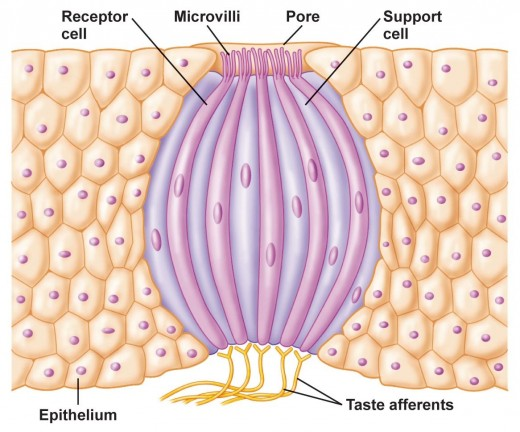
\includegraphics[width=8cm]{images/tastebud.jpg}
\caption{Taste Bud}
\label{fig: TBUD}
\end{figure}

\noindent \textbf{Gustatory Receptor Cells} are similar to most other cells. At the base of the receptor cell there is \textbf{a contact point}, a chemical synapse, with nerve fibers that respond to neurotransmitter molecules released by the taste receptor cells, initiating a signal that goes to the brain. The fibers carrying signals from taste receptor cells to the brain are part of the system of cranial nerves, notably cranial nerves 7, 9 and 10. \\

\noindent \textbf{Gustatory Cell Replacement:} Similar to the olfactory system,\textbf{ stem cells adjacent} to the taste receptor cells \textbf{can differentiate} into the \textbf{various types} of taste receptor cells, characterized by their \textbf{different taste receptor proteins}.This allows taste receptor cells to be \textbf{regularly replaced}, with a turnover rate of approximately two weeks. \\ 
This regular replacement is presumably related to the fact that gustatory and olfactory receptor cells are exposed to potentially toxic chemcials and subject to damage. \\

\newpage
\section{Five Taste Receptor Types:\\ Salt, Sour, Bitter, Sweet, and Umami}
Characterized by different kinds of taste receptor proteins.

\subsection{Salt}

\begin{itemize}
    \item Salt is Sodium Chloride (NaCl) and when in the mouth we experience the taste of saltiness. NaCl crystals in the mouth rapidly become Na$^+$ and Cl$^-$ ions in solution. 
    \item Proteins on taste receptor cells related to the perceptual experience of saltiness are thought to be \textbf{channels} that allow sodium ions to flow across the membrane. 
    \item When high (relatively) concentrations of Na$^+$ appear in the mouth after ingestion of salt, the Na$^+$ is believed to \textbf{flow through sodium ion channels} in the salt taste receptor cells, triggering a neural signal to the brain. 
    \item Sodium, potassium, calcium, and magnesium are essential cations for survival. 
    \item Taste of salt is experienced as pleasant. 
\end{itemize}

\subsection{Sour}

\begin{itemize}
    \item What we call "sour" is the taste of acids
    \item Citric acid from grapefruit and lemon, acetic acid from vinegar, lactic acid from sauerkraut and yogurt. 
    \item Defining feature of acids is the release of \textbf{hydrogen ions (H$^+$)} in solution. 
    \item Protein channels related to sour taste are sensitive to hydrogen ions. 
    \item When relatively high concentrations of H$^+$ appear in the mouth after ingestion of acidic substances, some kind of positive charge is believed to flow through \textbf{channels} in the sour taste receptor cells, triggering a neural signal to the brain. 
\end{itemize}

\subsection{Bitter}

\begin{itemize}
    \item \textbf{G-protein-coupled receptors (GPCRs)} initiate signals associated with the perceptual experience of bitterness 
    \item More than \textbf{30 different GPCR proteins} are distributed over the receptor cells associated with bitter taste. When a ligand binds to a GPCR, it initiates an intracellular signaling cascade leading to release of neurotransmitter and signal to the brain. 
    \item Diversity of GPCRs allows for a variety of different molecular shapes to be associated with the taste of bitterness. 
    \item Examples: caffeine, cocaine, morphine, and quinine (poisons) 
    \item Bitter taste may serve as a warning that item is poisonous. (Bitter-tasting things are common in nature) 
    \item However, we appreciate the taste of most bitter foods and aromas
\end{itemize}

\subsection{Sweet}

\begin{itemize}
    \item Defining taste of sugar is sucrose, table sugar. 
    \item Also glucose, fructose, lactose, maltose, and much more. (Hydrophilic C, O, H)
    \item Sweet receptor proteins are also \textbf{GPCRs} 
    \item Two distinct GPCRs for sweet tasting detection 
        \subitem The particular molecular shapes of the various sugar molecules permit them to bind as ligands to the sweet GPCRs, shape-shift the proteins, and initiate a signal. (similar encodings and shapes) 
        \subitem The functional form of the sweet taste receptor protein appears to be a \textit{dimer} of two GPCRs, that is, the two GPCRs are linked (noncovalent interaction) to form the functional sweet receptor. (basically two GPCRs smashed together and can either be two of the same type of two different types of sugar GPCRs) 
        \subitem GPCR multimers exist as well (multiple GPCRs smashed together) 
    \item Max Delbruck(1906-1981):  \textbf{"Principle of Limited Sloppiness"} (1950)
        \subitem Used to describe situations in experimental research where unexpected discoveries are made because a scientist is a little sloppy, but not so sloppy to not figure out what happened. 
        \subitem How the discovery of artificial sugars came to be. 
\end{itemize}

\noindent \textbf{Sweeter-than-Sugar Sweeteners}: 
\begin{itemize}
    \item Saccharin:(synthetic and artificial) 500x sweeter than sucrose
    \item Aspartame:(synthetic and artificial) 180x sweeter than sucrose
    \item Stevioside:(\textit{Stevia rebaudiana} plant in Amazon jungle of South America) 300x sweeter than sucrose 
    \item Sucralose:(synthetic and artificial) 600x sweeter than sucrose. 3 OH groups in sucrose replaced with Cl (aka Splenda)
        \subitem (2004 - 2007) Equal sues Splenda company, claiming false advertising: "there is no sugar in Splenda and Splenda's sweet taste does not come from sugar"
    \item Neotame:(synthetic and artificial) 10000x sweeter than sucrose. 
        \subitem How diet drinks are made (with these other sugars as well). Little sugar molecules make calories almost 0 (taken from aspartame) approved by FDA in 2002
\end{itemize}

\subsection{Umami}

\begin{itemize}
    \item Discovered in 1909 by Japanese chemist Kikunae Ikeda (1864-1936) at University of Tokyo, Japan
    \item Receptor cell responds to glutamate with metabotropic GPCR glutamate receptors as taste receptors. 
    \item Responsible for "savory", "meaty", "delicious" taste
    \item \textit{Umai}: Delicious, \textit{mi}: Taste
    \item Americans and Europeans continued to speak of 4 tastes until the 1990s
    \item Umami taste receptor cloned in 2000
    \item Glutamate is an amino acid - where there is protein, there is glutamate
    \item Umami receptors also respond to other amino acids present in protein. 
\end{itemize}

\newpage
\section{Gustatory Neural Pathways}

Cranial nerve fivers carrying taste sensory information enter the brain via the lower brainstem and connect with cells in the nucleus solitarius. \\
Two axon tracts emerge: \\
\indent One heading to the \textbf{thalamus} and thence to the \textbf{insula} and to the \textbf{somatosensory cortex} in the parietal lobe \\
\indent Other heading to the \textbf{hypothalamus} and \textbf{amygdala} \\
Somehow related to our perception of food qualities and tastes. \\

\subsection{Spiciness}

\begin{itemize}
    \item The quality of hotness, spiciness or pungency
    \item Most notable items to cause are black pepper, chili, mustard, horseradish, wasabi, ginger, and garlic
    \item Activate various receptors in the mouth that relate to pain. Fifth cranial nerve (trigeminal nerve)
    \item Reason why spiciness is not considered a taste
\end{itemize}

\subsection{Capsaicin}

The chili plant \textit{Capsicum annuum}, native to South America, is known for it's spicy hotness. Includes plants such as cayenne, jalapeno, pimento, habanero, etc. Unknown to the world until voyages by explorers like Christopher Columbus. 

\begin{itemize}
  \item Hotness of chili associated with single molecular constituent - \textbf{Capsaicin}
  \item The more capsaiin present, the hotter it is perceived
  \item When capsaicin binds to one of these receptor proteins, a shape change occurs, an \textbf{ion channel opens}, and \textbf{calcium ions flow} from \textit{outside} the cell \textit{to inside}, \textbf{depolarizing} the cell and leading to increased neural excitability. 
  \item Thermal heat also activates capsaicin-sensitive proteins by causing some kind of shape change with increase of temperature. 
  \item Chili hot and fire hot are perceived using same molecular and cellular mechanisms. 
  \item Capsaicin receptor proteins are all over our body as well. 
\end{itemize}

\subsection{Hot vs. Cold}

Capsaicin receptors became known as members of a large family of ionotropic proteins (characterized by study of fruit fly vision) known as \textbf{TRP Channels}. \\

\textbf{Transient Receptor Potential (TRP):}
\begin{itemize}
    \item A reference to an electrical response of the insect eye to light
    \item Capsaicin receptor is now known by \textbf{TRPVI}
    \item Its \textbf{ion channel opens} in response to capsaicin and also to heat in the temperature range of 43-50 degrees Celsius (109-122 degree Fahrenheit). 
    \item Piperine also opened TRPVI channels, a molecule found in black pepper (\textit{Piper nigrum})
\end{itemize}

Separate signaling pathway for cold. Characterized by using a molecule from mint plants \textbf{menthol} \\

\textbf{Menthol:}
\begin{itemize}
    \item Appreciated for its distinctive flavor qualities, perceived as coolness
    \item \textbf{Ionotropic receptor} protein found in mouth and elsewhere in which a calcium channel opens in response to the binding of menthol
    \item Temperatures cooler (8-28 degrees Celsius or 46-82 degrees Fahrenheit than body temperature (37 degrees Celsius) produce a shape change of this protein and open the channel. 
    \item Analogous to capsaicin and heat, these receptors also respond to cool temperatures.
    \item Also member of TRP receptor family, known as \textbf{TRPM8}
\end{itemize}

\subsection{Isothiocyanates}

Associated with perceptual quality of hotness is a family of molecules known as the isothiocyanates, characterized by a particular configuration of sulfur, carbon and nitrogen atoms.

\begin{itemize}
    \item Ionotropic Ca$^++$ channel called \textbf{TRPA1}
    \item Activated by the binding of isothiocyanates
    \item Results in neural signals different from capsaicin and TRPV1, associated with experiences of hotness and pungency
    \item mustard, horseradish, wasabi
\end{itemize}

\newpage
\section{Flavor}
\begin{itemize}
    \item Combination of several different channels of sensory information 
    \item The mouth components of taste and pungency are hugely important to the flavor of food and drink: salty, sour, sweet, bitter, umami, cool and several kinds of spicy hot 
    \item Texture contributes to flavor. 
    \item Aromatic molecules sensed via olfactory system contributes to flavor the most. 
\end{itemize}



\newpage
George Berkeley (1685 - 1753) \\
A Treatise Concerning the Principles of Human Knowledge (1710) \\
All we know is our perception, the entire world is created by our perception. \\
Coming to the limits of what we can say about human consciousness. \\
spent last lecture talking about olfactory sensors/bulbs \\

Stem cells and gustatory cell replacement

FLAVOR: 
    Taste
    Smell
    Pungency
    Texture
    
Taste receptor cell types: 
    believed that ion channels have something to do with taste
    salt
        ion channel sensitive to Na$^+$    
    sour
        ion channel sensitive to H$^+$ (acids taste sour)
    bitter
        30 GPCRs, encode for bitter taste. 
        Many different molecules (different shapes) found in nature taste bitter 
        (There is only one salt (i think) but many things can taste bitter. various bitter plant alkaloids: 
            caffeine
            quinine
            cocaine
            absinthin (absinth alcohol must get some)
    sweet
        2 GPCRs encode for sweet taste
        the molecules for sweet stuff have similar encodings and shapes
        GPCR dimer (two gpcr smashed together, with either the same gpcrs or different gpcrs
        gpcr multimers are a thing as well. 
        "sugar"
            sucrose (C, O, H hydrophilic)
            glucose
            fructose
            originated in SE Asia and South Pacific and reached Mediterranean in 1000BC
            Honey (original sugar source) as well as fruits
            saccharin (500x) (man made) (synthetic and artificial)
            aspartame (180x) (man made) (synthetic and artificial)
            stevioside (300x sweeter than sucrose) from stevia rebaudiana
            Max Delbruck (1906 - 1981) - Principle of Limited Sloppiness 1950 (how saccharin and aspartame were discovered)
            sucralose (600x) with sucrose, 3 OH groups replaced with Cl (splenda)
                2004 -2007 (equal sues splenda company, claiming false advertising: "there is no sugar in splenda and splenda's sweet taste does not come from sugar)
            Neotame (10000x) (how diet drinks are made. Little sugar molecules make calories almost 0) (taken from aspartame) approved by FDA in 2002
        Artificial sugars no good for you
        Miracle Fruit (synsepalum dulcificum) West Africa
            miraculin protein 199 amino acids
            binds to sweet reeptor gpcr dimer
            makes sour things taste sweet
            strong agonist effects only at highly acidic pH
    umami 
        "delicious", "savory", glutamate related to this savory taste
        GPCR, similar to the ones in our brains (glutamate receptors)
        related to cooked meats and mushrooms anything that has the burst of umami
        discovered in 1909 by Kikunae Ikeda of Imperial University of Tokyo, Japan
        Americans and Europeans continued to speak of 4 tastes until the 1990s
        umami taste receptor cloned in 2000
    Discussion of taste receptor for fats
    
    Chili peppers (capsicum annum) South America
        Cayenne
        Bell pepper (same species as cayenne)
            pepper: after asian pepper
        pasilla
        habenero (capsicum chinense)
        concentrations of capsaicin ("hot" substance in chili)
            why hot?
            capsaicin receptor a heat-activated ion channel in the pain pathway
            open Ca$^++$ channel, depolarization
            signals temperature hot, pain
            
            
Microvilli containing taste proteins
 
    




\end{document}